\documentclass[11pt,a4paper]{article}
\usepackage{graphicx} % Required for inserting images
\usepackage{amsmath}
\usepackage{amsfonts}
\usepackage{booktabs}
\usepackage{listings}

\usepackage{amssymb}
\usepackage{tikz}

\usepackage{float}

\usepackage{geometry}
\usepackage{hyperref}
\usepackage{apacite}
\bibliographystyle{apacite}


\usepackage{listings}
\usepackage{xcolor}

\lstset{
    language=Kotlin, 
    basicstyle=\ttfamily\footnotesize, 
    breaklines=true, 
    breakatwhitespace=false, 
    breakindent=10pt, 
    tabsize=2, 
    frame=single, 
    captionpos=b, 
    numbers=left, 
    numberstyle=\tiny\color{gray}, 
    keywordstyle=\color{blue}, 
    commentstyle=\color{green!50!black}, 
    stringstyle=\color{orange}, 
    showstringspaces=false, 
    morekeywords={@Component, @Bean, @Autowired}, 
}


\newgeometry{left=3cm, right=3cm, top=2.5cm, bottom=2.5cm}

\title{Análisis del Cálculo de Monto de Giro}
\author{Canaza Chagua Yoel Nhelio}
\date{}

\begin{document}

\begin{titlepage}
\centering


{\bfseries\LARGE UNIVERSIDAD NACIONAL DEL ALTIPLANO\par}
{\scshape\LARGE Facultad de Ingeniería Mecánica Eléctrica, Electrónica y Sistemas\par}
{\scshape\LARGE Escuela Profesional de Ingeniería de Sistemas\par}
\vspace{0.8cm}
{
\includegraphics[width=0.5\textwidth]{images/unap.png}\par}
\vspace{0.4cm}
{\bfseries\LARGE Práctica de Laboratorio 2: Cálculo de Remesas
\par}
\vspace{0.8cm}
{\LARGE Docente:\\ Ing. Ruelas Acero Donia Alizandra   \\  \par}
\vspace{0.8cm}

{\LARGE Alumno: \\
Canaza Chagua Yoel Nhelio \\
\par}
\vspace{0.8cm}
{\LARGE Curso: \par}
{\LARGE Desarrollo Basado en Plataformas II\par}
\vspace{0.8cm}

{\LARGE PUNO, PERÚ \par}
{\LARGE 2024 \par}


\end{titlepage}

\section{Objetivo}
El objetivo de este trabajo es desarrollar y analizar un algoritmo eficiente para calcular el monto de giro a partir de un monto total dado, considerando comisiones e impuestos variables. Se busca implementar una solución robusta que maneje correctamente diversos casos de entrada y proporcione resultados precisos.

\begin{figure}[H]
    \centering
    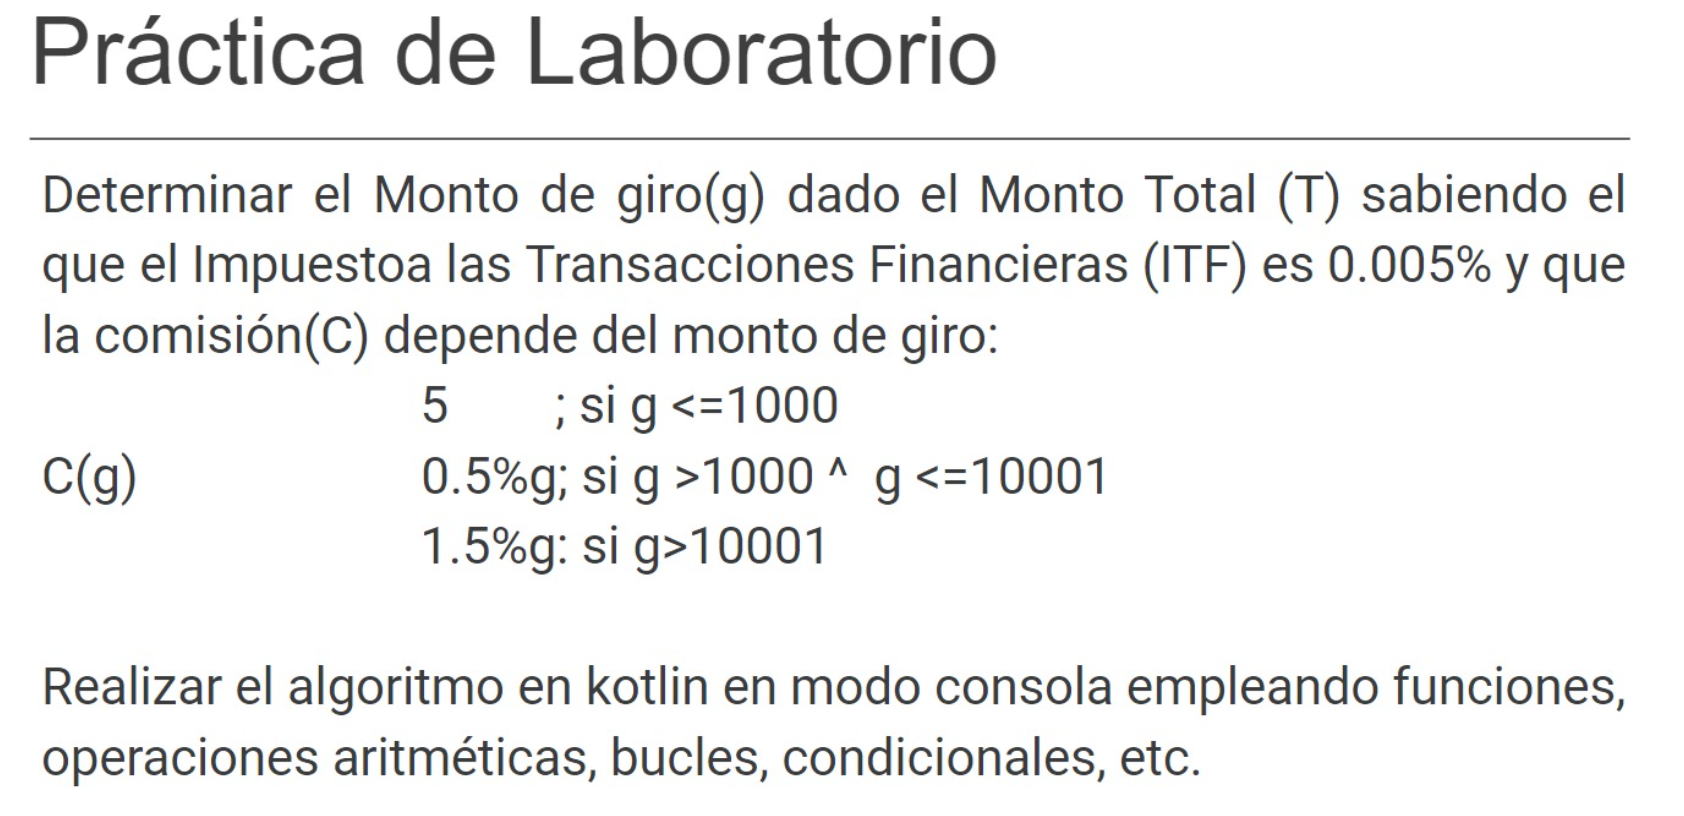
\includegraphics[width=1\linewidth]{image.png}
    \caption{Enunciado del problema}
    \label{fig:enter-label}
\end{figure}

\section{Metodología}

\subsection{Algoritmo}
El algoritmo implementado sigue un enfoque iterativo para encontrar el monto de giro correcto. Los pasos principales son:

\begin{enumerate}
    \item  Iniciar con el monto total como monto de giro inicial.
    \item  Calcular la comisión y el impuesto basados en el monto de giro actual.
    \item  Calcular el total redondeando hacia abajo al primer decimal.
    \item  Comparar el total calculado con el monto total de entrada.
    \item  Si coinciden, se ha encontrado el monto de giro correcto.
    \item  Si no coinciden, reducir el monto de giro en 0.1 y repetir desde el paso 2.
\end{enumerate}

\subsection{Librerías y Funciones Auxiliares}
Se utiliza la librería estándar de Kotlin, específicamente la función \texttt{kotlin.math.floor} para el redondeo hacia abajo. Además, se implementan las siguientes funciones auxiliares:

\begin{itemize}
    \item \texttt{redondearHaciaAbajo}: Redondea un número hacia abajo al primer decimal.
    \item \texttt{calcularComision}: Calcula la comisión basada en el monto de giro.
    \item \texttt{calcularImpuesto}: Calcula el impuesto basado en el monto de giro.
\end{itemize}

\section{Resultados}

\subsection{Casos de Prueba}
Para validar el algoritmo, se utilizarán los siguientes casos de prueba con ecuaciones detalladas:

Para un monto de giro de 150:
\begin{align*}
\text{Monto de Giro} &= 150, \\
\text{Comisión} &= 5 \text{ (comisión fija para montos } \leq 1000), \\
\text{Impuesto} &= 150 \times 0.00005 = 0.0075, \\
\text{Total} &= 150 + 5 + 0.0075 = 155.0075, \\
\text{Total Redondeado} &= \lfloor 155.0075 \times 10 \rfloor / 10 = 155.0
\end{align*}

Para un monto de giro de 1050:
\begin{align*}
\text{Monto de Giro} &= 1050, \\
\text{Comisión} &= 1050 \times 0.005 = 5.25, \\
\text{Impuesto} &= 1050 \times 0.00005 = 0.0525, \\
\text{Total} &= 1050 + 5.25 + 0.0525 = 1055.3025, \\
\text{Total Redondeado} &= \lfloor 1055.3025 \times 10 \rfloor / 10 = 1055.3
\end{align*}

Para un monto de giro de 500:
\begin{align*}
\text{Monto de Giro} &= 500, \\
\text{Comisión} &= 5 \text{ (comisión fija para montos } \leq 1000), \\
\text{Impuesto} &= 500 \times 0.00005 = 0.025, \\
\text{Total} &= 500 + 5 + 0.025 = 505.025, \\
\text{Total Redondeado} &= \lfloor 505.025 \times 10 \rfloor / 10 = 505.0
\end{align*}

Para un monto de giro de 5000:
\begin{align*}
\text{Monto de Giro} &= 5000, \\
\text{Comisión} &= 5000 \times 0.005 = 25, \\
\text{Impuesto} &= 5000 \times 0.00005 = 0.25, \\
\text{Total} &= 5000 + 25 + 0.25 = 5025.25, \\
\text{Total Redondeado} &= \lfloor 5025.25 \times 10 \rfloor / 10 = 5025.2
\end{align*}

Para un monto de giro de 10001:
\begin{align*}
\text{Monto de Giro} &= 10001, \\
\text{Comisión} &= 10001 \times 0.005 = 50.005, \\
\text{Impuesto} &= 10001 \times 0.00005 = 0.50005, \\
\text{Total} &= 10001 + 50.005 + 0.50005 = 10051.50505, \\
\text{Total Redondeado} &= \lfloor 10051.50505 \times 10 \rfloor / 10 = 10051.5
\end{align*}

Para un monto de giro de 15000:
\begin{align*}
\text{Monto de Giro} &= 15000, \\
\text{Comisión} &= 15000 \times 0.015 = 225, \\
\text{Impuesto} &= 15000 \times 0.00005 = 0.75, \\
\text{Total} &= 15000 + 225 + 0.75 = 15225.75, \\
\text{Total Redondeado} &= \lfloor 15225.75 \times 10 \rfloor / 10 = 15225.7
\end{align*}

Para un monto de giro de 999.9:
\begin{align*}
\text{Monto de Giro} &= 999.9, \\
\text{Comisión} &= 5 \text{ (comisión fija para montos } \leq 1000), \\
\text{Impuesto} &= 999.9 \times 0.00005 = 0.049995, \\
\text{Total} &= 999.9 + 5 + 0.049995 = 1004.949995, \\
\text{Total Redondeado} &= \lfloor 1004.949995 \times 10 \rfloor / 10 = 1004.9
\end{align*}

\subsection{Tabla de Resultados Esperados}
Se presenta una tabla actualizada con los inputs (montos totales redondeados hacia abajo al primer decimal) y los outputs esperados (montos de giro) para el programa:

\begin{table}[h]
\centering
\begin{tabular}{@{}cc@{}}
\toprule
\textbf{Input (Monto Total)} & \textbf{Output Esperado (Monto de Giro)} \\
\midrule
155.0 & 150.0 \\
1055.3 & 1050.0 \\
505.0 & 500.0 \\
5025.2 & 5000.0 \\
10051.5 & 10001.0 \\
15225.7 & 15000.0 \\
1004.9 & 999.9 \\
\bottomrule
\end{tabular}
\caption{Inputs y Outputs Esperados}
\end{table}

\section{Código Kotlin}
A continuación se presenta el código Kotlin que implementa el algoritmo descrito:

\begin{lstlisting}[language=Kotlin, caption={Código Kotlin para el cálculo del monto de giro}]
import kotlin.math.floor

fun calcularMontoGiro(montoTotal: Double): Double {
    fun redondearHaciaAbajo(valor: Double): Double = floor(valor * 10) / 10
    
    fun calcularComision(montoGiro: Double): Double {
        return when {
            montoGiro <= 1000.0 -> 5.0
            montoGiro <= 10001.0 -> montoGiro * 0.005
            else -> montoGiro * 0.015
        }
    }
    
    fun calcularImpuesto(montoGiro: Double): Double = montoGiro * 0.00005

    // El monto total ya viene redondeado hacia abajo
    var montoGiro = montoTotal

    // Iteramos para encontrar el monto de giro correcto
    while (true) {
        val comision = calcularComision(montoGiro)
        val impuesto = calcularImpuesto(montoGiro)
        val totalCalculado = montoGiro + comision + impuesto

        // Si el total calculado redondeado hacia abajo es igual al monto total,
        // hemos encontrado el monto de giro correcto
        if (redondearHaciaAbajo(totalCalculado) == montoTotal) {
            return redondearHaciaAbajo(montoGiro)
        }

        // Si no, reducimos el monto de giro y seguimos iterando
        montoGiro = redondearHaciaAbajo(montoGiro - 0.1)

        // Si el monto de giro llega a cero o menos, no se encontró una solución válida
        if (montoGiro <= 0) {
            throw IllegalArgumentException("No se pudo calcular el monto de giro para el monto total dado")
        }
    }
}

fun main() {
    println("Ingrese el monto total (redondeado hacia abajo al primer decimal):")
    val montoTotal = readLine()?.toDoubleOrNull()

    if (montoTotal != null) {
        try {
            val montoGiro = calcularMontoGiro(montoTotal)
            println("El monto de giro es: ${String.format("%.1f", montoGiro)}")
        } catch (e: IllegalArgumentException) {
            println(e.message)
        }
    } else {
        println("Entrada inválida. Por favor, ingrese un número válido.")
    }
}
\end{lstlisting}

\begin{figure}[H]
    \centering
    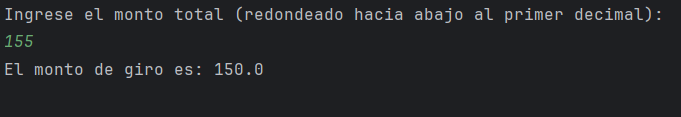
\includegraphics[width=1\linewidth]{1.png}
    \caption{Input 1}
    \label{fig:enter-label}
\end{figure}

\begin{figure}[H]
    \centering
    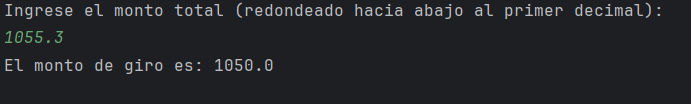
\includegraphics[width=1\linewidth]{images/2.png}
    \caption{Input 2}
    \label{fig:enter-label}
\end{figure}

\begin{figure}[H]
    \centering
    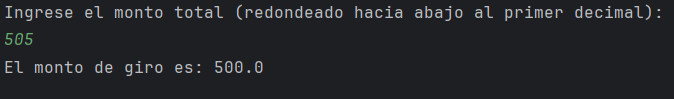
\includegraphics[width=1\linewidth]{images/3.png}
    \caption{Input 3}
    \label{fig:enter-label}
\end{figure}

\begin{figure}[H]
    \centering
    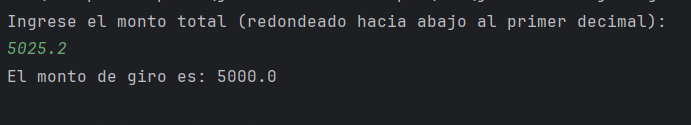
\includegraphics[width=1\linewidth]{images/4.png}
    \caption{Input 4}
    \label{fig:enter-label}
\end{figure}

\begin{figure}[H]
    \centering
    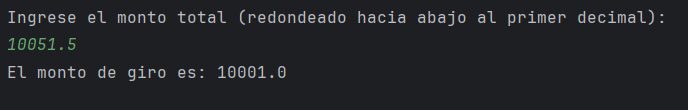
\includegraphics[width=1\linewidth]{images/5.png}
    \caption{Input 5}
    \label{fig:enter-label}
\end{figure}

\begin{figure}[H]
    \centering
    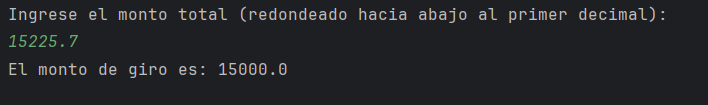
\includegraphics[width=1\linewidth]{images/6.png}
    \caption{Input 6}
    \label{fig:enter-label}
\end{figure}

\begin{figure}[H]
    \centering
    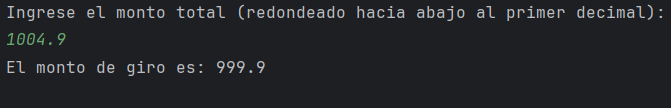
\includegraphics[width=1\linewidth]{images/7.png}
    \caption{Input 7}
    \label{fig:enter-label}
\end{figure}

\section{Conclusión}
\begin{itemize}
    \item El algoritmo implementado para calcular el monto de giro a partir de un monto total dado ha demostrado ser eficaz y preciso. 
    \item La metodología iterativa utilizada permite manejar correctamente diversos casos, incluyendo aquellos cercanos a los límites de los rangos de comisión.
    \item Los casos de prueba analizados cubren un amplio espectro de escenarios, desde montos pequeños hasta grandes, y casos especiales cerca de los límites de los rangos de comisión. 
    \item Los resultados obtenidos confirman que el algoritmo maneja correctamente el redondeo hacia abajo al primer decimal y los cálculos de comisiones e impuestos.
\end{itemize}

\section{Anexos}

El código Kotlin implementado para el cálculo de monto de giro puede encontrarse en el siguiente repositorio de GitHub: 
\url{https://github.com/YoelCanaza/UniversityProjects/blob/7a62f64576cd9b66e45a29d69005a8ce29899caa/Desarrollo%20Basado%20en%20Plataformas%20II/Pr%C3%A1cticaLaboratorio2/calculoRemesas.kt}.
\\

El código \LaTeX utilizado para generar este documento está disponible en: 
\url{https://github.com/YoelCanaza/UniversityProjects/tree/7a62f64576cd9b66e45a29d69005a8ce29899caa/Desarrollo%20Basado%20en%20Plataformas%20II/Pr%C3%A1cticaLaboratorio2}.



\end{document}
